% bare_jrnl_compsoc, texV1.4b, 2015/08/26, Michael Shell
\documentclass[10pt,journal,compsoc]{IEEEtran}

% *** MISC UTILITY PACKAGES ***

\newcommand{\note}[1]{\textcolor{magenta}{#1}} 
\usepackage[nocompress]{cite}
\usepackage[]{footmisc}
\usepackage{hyperref} % autoref
% *** GRAPHICS RELATED PACKAGES ***
\ifCLASSINFOpdf
   \usepackage[pdftex]{graphicx}
  % declare the path(s) where your graphic files are
   \graphicspath{{./figures/}}
  % and their extensions so you won't have to specify these with
  % every instance of \includegraphics
  % \DeclareGraphicsExtensions{.pdf,.jpeg,.png}
\else
  % or other class option (dvipsone, dvipdf, if not using dvips). graphicx
  % will default to the driver specified in the system graphics.cfg if no
  % driver is specified.
   \usepackage[dvips]{graphicx}
  % declare the path(s) where your graphic files are
   \graphicspath{{./figures/}}
  % and their extensions so you won't have to specify these with
  % every instance of \includegraphics
   \DeclareGraphicsExtensions{.eps}
\fi

% latex, and pdflatex in dvi mode, support graphics in encapsulated
% postscript (.eps) format. pdflatex in pdf mode supports graphics
% in .pdf, .jpeg, .png and .mps (metapost) formats. Users should ensure
% that all non-photo figures use a vector format (.eps, .pdf, .mps) and
% not a bitmapped formats (.jpeg, .png). The IEEE frowns on bitmapped formats
% which can result in "jaggedy"/blurry rendering of lines and letters as
% well as large increases in file sizes.

% *** MATH PACKAGES ***
%% with other math-related packages, you may want to disable it.
\usepackage{amsmath, amsthm, amsfonts,amssymb,eulervm,xspace, mathtools}
\renewcommand{\restriction}{\mathord{\upharpoonright}} %restriction w/p space
\usepackage{mathrsfs} % math script fonts
\usepackage{relsize} %bigger
\usepackage{bm}
\theoremstyle{definition}
\newtheorem{definition}{Definition}[section]
\theoremstyle{remark}
\newtheorem{example}{Example}[section]
% *** SPECIALIZED LIST PACKAGES ***
\usepackage{xcolor}
\usepackage{algorithmic}
\usepackage[utf8]{inputenc}
\usepackage{subfig} %ieee does not like subfigure
\usepackage{multicol}
\usepackage{tikz}
\usetikzlibrary{cd} % commutative diagrams
\newtheorem{prop}{Proposition} %math?
\usepackage[switch]{lineno}
\renewcommand{\linenumberfont}{\normalfont\bfseries\small\color{lightgray}}
\usepackage{minted}
\setminted[python]{fontsize=\scriptsize, 
                   linenos,
                   numbersep=8pt,
                   autogobble, 
                   frame=lines,
                   framesep=3mm} 
% *** ALIGNMENT PACKAGES ***
\usepackage{array}
\usepackage{tabulary}
% IEEEtran contains the IEEEeqnarray family of commands

% *** SUBFIGURE PACKAGES ***
\ifCLASSOPTIONcompsoc
  \usepackage[caption=false,font=footnotesize,labelfont=sf,textfont=sf]{subfig}
\else
  \usepackage[caption=false,font=footnotesize]{subfig}
\fi

% *** FLOAT PACKAGES ***
\usepackage{dblfloatfix}

% *** PDF, URL AND HYPERLINK PACKAGES ***
\usepackage{url}

% *** Do not adjust lengths that control margins, column widths, etc. ***
% *** Do not use packages that alter fonts (such as pslatex).         ***
% There should be no need to do such things with IEEEtran.cls V1.6 and later.
% (Unless specifically asked to do so by the journal or conference you plan
% to submit to, of course. )

\usepackage{notation} %notation conventions
% correct bad hyphenation here
\hyphenation{op-tical net-works semi-conduc-tor}



\begin{document}
\linenumbers

\title{Topological Equivariant Artist Model for Visualization Library Architecture}
% author names and IEEE memberships
\author{Hannah~Aizenman, Thomas~Caswell, and~Michael~Grossberg,~\IEEEmembership{Member,~IEEE,}% <-this % stops a space
\IEEEcompsocitemizethanks{\IEEEcompsocthanksitem H. Aizenman and M. Grossberg are with the department of Computer Science, City College of New York. 
\protect\\
% note need leading \protect in front of \\ to get a newline within \thanks as
% \\ is fragile and will error, could use \hfil\break instead.
E-mail: haizenman@ccny.cuny.edu, mgrossberg@ccny.cuny.edu 
\IEEEcompsocthanksitem Thomas Caswell is with National Synchrotron Light Source II, Brookhaven National Lab 
\protect \\
E-mail: tcaswell@bnl.gov}% <-this % stops an unwanted space
\thanks{Manuscript received X XX, XXXX; revised X XX, XXXX.}
}


% for Computer Society papers, we must declare the abstract and index terms
% PRIOR to the title within the \IEEEtitleabstractindextext IEEEtran
% command as these need to go into the title area created by \maketitle.
% As a general rule, do not put math, special symbols or citations
% in the abstract or keywords.
\IEEEtitleabstractindextext{%
\begin{abstract}
The abstract goes here.
\end{abstract}

% Note that keywords are not normally used for peerreview papers.
\begin{IEEEkeywords}
%Computer Society, IEEE, IEEEtran, journal, \LaTeX, paper, template.
\end{IEEEkeywords}}


% make the title area
\maketitle


\IEEEpeerreviewmaketitle



\IEEEraisesectionheading{\section{Introduction}\label{sec:intro}}


\IEEEPARstart{T}

\section{Related Work}

\section{Expressing Structure}
\label{sec:atct}
\note{why why why?}
We use concepts from algberaic topolology and category theory to formally express the structure visualization components are expected to preserve.  Fiber bundles and sheaves, which come from algebraic topolology, provide a uniform generalizable way to describe data and visualizations. Category theory is a method to describe how objects are specified, constrained, and composed \cite{wielsManagementEvolvingSpecifications1998}\; therefore in this work we propose categorical constructions of visualization components as specifications for implementable components.

\subsection{Fiber Bundles}
\label{sec:atct:fiber-bundles}
Fiber bundles, are a "unified, dimension-independent framework", as described by Butler\cite{butlerVectorBundleClassesForm1992,butlerVisualizationModelBased1989}, that allow us to seperatly describe the topololigical properties and fields of a data source and also the mapping between topolology and data values. A fiber bundle $(\dtotalc, \dbasec, \pi, \dfiberc)$ is a structure with topological spaces $\dtotalc, \dfiberc, \dbasec$ and continuous surjective map $\pi: \dtotalc \rightarrow \dbasec$\cite{FiberBundle2020}. 

\begin{equation}
  \label{eq:atct:fb_intro}
  \begin{tikzcd}[ampersand replacement=\&, row sep=huge]
   \dfiberc
    \arrow[r, hook] \& 
    \dtotalc
    \arrow[d, "\pi"'] \\
     \& 
  \dbasec
     \arrow[u, "\dsectionc"', bend right, pos=.5]
  \end{tikzcd}
\end{equation} 


The \textcolor{base}{base space} is a topological space \dbasec\ with points $\dbasepointc \in \dbasec$ and topology $\mathcal{T}_{\dbasec}$; $\mathcal_{T}_k$ is a set of opensets $ \dbasepointc \in \opensetc \subseteqq \dbasec$ \cite{munkresElementsAlgebraicTopology1984} that cover the base space \dbasec.  The \textcolor{fiber space} is a topological space \dfiberc\ that is the preimage of the projection function $\pi$ at a point in the base space $\dfiberc|_{\dbasepointc} = \pi^{-1}(\dbasepointc)$ and fibers of a bundle are isomorphic $\dfiberc \simeq \dfiberc_{\dbasepointc}\;\forall \dbasepointc \in \dbase$. The \textcolor{section}{sections} of a bundle $\dsection$ are maps from the base space to points in the bundles over that base space and $\textcolor{set}{\Gamma}$ denotes the set of all sections in a bundle over an openset. 
\begin{equation}
  \label{eq:atct:fb_sections}
  \cgamma{\opensetgc}{\gtotalc\restriction_{\opensetgc}} \coloneqq \big\{\gsectionc: \opensetgc\rightarrow \gtotalc\restriction_{\opensetgc} \; \bigm{\vert} \pi(\gsectionc(\gbasepointc)) = \gbasepointc\;for\, all\; \gbasepointc \in \opensetgc \big\} 
\end{equation}
 
A fiber bundle is locally trivial, which means that for every point \dbasepointc\ there exists an open neighborhood $\dbasepointc \in \opensetc \subseteq \dbasec$ such that there is a homeomorphism $\pi^{-1}(\opensetc)\xrightarrow{\equivc} \opensetc \times \dfiberc$. A bundle may be globally trivial, meaning that $\dtotalc = \dbasec \times \dfiberc$, and generally can be thought of as a twisted product of total and base spaces \cite{munkresElementsAlgebraicTopology1984}. 

\begin{figure}
  \label{fig:atct:fb}
  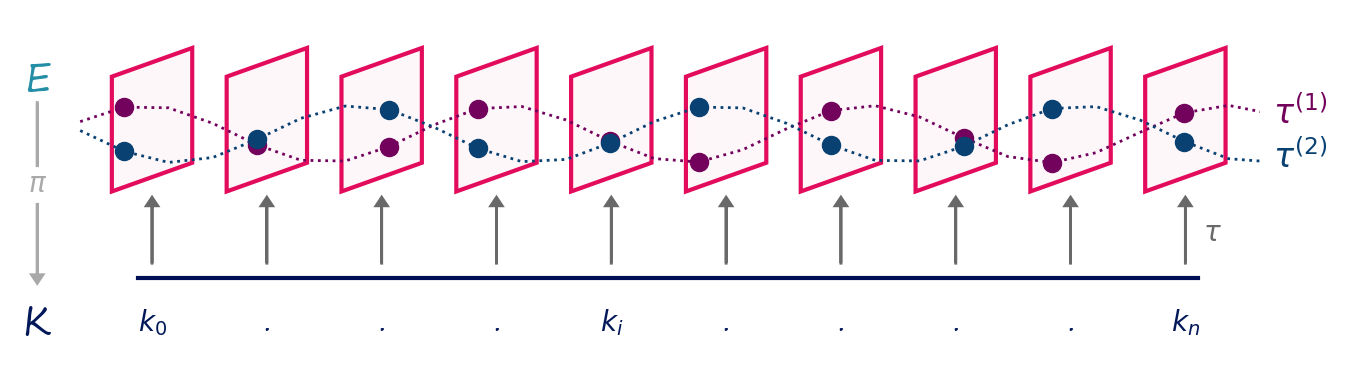
\includegraphics[width=\columnwidth]{fiberbundle.png}
  \caption{change to concrete example}
\end{figure}

Fiber bundles can be used to model data for visualization, as proposed by Butler\cite{butlerVectorBundleClassesForm1992, butlerVisualizationModelBased1989}. We encode the topological properties of the data \cite{wilkinsonGrammarGraphics2005} as the base space \dbasec. The topological properties, as described by Wilkenson, are how the data is organized - for example \dbase\ could be discrete points, a line, a 2D surface, a 3D volume, or a graph. The names and data types of the data fields can be expressed as the fiber space \dfiberc, as described by Spivak \cite{spivakDatabasesAreCategories2010,spivakSIMPLICIALDATABASES}. For example, a temperature field could be expressed as a fiber $\dfiber_{temperature}=\mathbb{R}$, and a color field could be $\dfiber_{color}=\mathbb{R}^{3}$. Even though fibers on non-trivial spaces, such as vector fields, are different, we can simplify to one type because fibers are isomorphic.\note{unsure of this claim but I think this is why, and also I need to tell you why you care that they're isomorphic} The total bundle space \dtotalc\ acts as a way of expressing all data with the same topolology \dbasec\ and fields \dfiberc, for example a database schema. A specific dataset is represented as a section \dsectionc, and the return values of a section evaluated at a point \dbasepointc\ is the record $\{field_{0}: value_{0}, ..., field_n:value_n\}$ at that point. 

\begin{figure}
  \label{fig:atct:fb_graphic_bundle}
  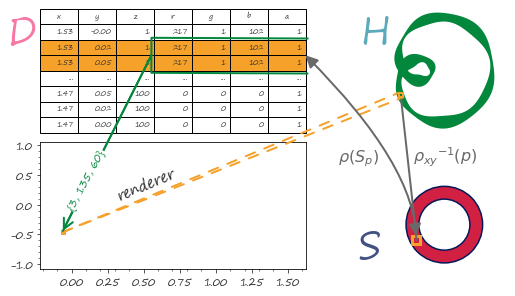
\includegraphics[width=1\columnwidth]{render.png}
  \caption{}
\end{figure}

We also use fiber bundles to represent the output of a visualization algorithm, which we term the graphic but generalizes to output on any display space, such as a screen or 3D print. 
\begin{equation}
  \label{eq:atct:fb_graphic}
  \gfiberc \hookrightarrow \gtotalc \xrightarrow{\pi} \gbasec
\end{equation}
The base space \gbasec\ is a parameterization of the display area, for example the inked bounding box in cairo \cite{CairographicsOrg}. The fiber space \gfiberc\ is an abstraction of the renderer fields, for example $\{x,\,y,\,r,\,g,\,b,\,a\}$. The sections of the graphic 
\begin{equation}
  \label{eq:atct:fb_graphic_section}
  $\cgamma{\opensetgc}{\gtotalc\restriction_{\opensetgc}} \coloneqq \big\{\gsectionc: \opensetgc\rightarrow \gtotalc\restriction_{\opensetgc} \; \bigm{\vert} \pi(\gsectionc(\gbasepointc)) = \gbasepointc\;for\, all\; \gbasepointc \in \opensetgc \big\}$
\end{equation}
are functions that generate different graphics, for example markers for a scatter plot, bars for a bar chart, cells of a heatmap, or pixels of an image.

\subsubsection{Input and Output Types}

\subsection{Sheaves}
Sheaves on bundles are an "algebraic data structure", as described by Ghrist \cite{ghristElementaryAppliedTopology2014}, for expressing the bookkeeping involved in subsetting data and composing data that is distributed or streaming. 

\subsection{Transforms on Sheaves}

\subsection{Transforms Between Sheaves}

\section{Preserving Structure}





\section{Discussion}
\subsection{Limitations}
\subsection{future work}

\section{Conclusion}
The conclusion goes here.


\appendices
\section{Category Theory}
\subsection*{Category}
\subsection*{}



% use section* for acknowledgment
\ifCLASSOPTIONcompsoc
  % The Computer Society usually uses the plural form
  \section*{Acknowledgments}
\else
  % regular IEEE prefers the singular form
  \section*{Acknowledgment}
\fi


The authors would like to thank...


% Can use something like this to put references on a page
% by themselves when using endfloat and the captionsoff option.
\ifCLASSOPTIONcaptionsoff
  \newpage
\fi

% trigger a \newpage just before the given reference
% number - used to balance the columns on the last page
% adjust value as needed - may need to be readjusted if
% the document is modified later
%\IEEEtriggeratref{8}
% The "triggered" command can be changed if desired:
%\IEEEtriggercmd{\enlargethispage{-5in}}

% references section

% can use a bibliography generated by BibTeX as a .bbl file
% BibTeX documentation can be easily obtained at:
% http://mirror.ctan.org/biblio/bibtex/contrib/doc/
% The IEEEtran BibTeX style support page is at:
% http://www.michaelshell.org/tex/ieeetran/bibtex/
\bibliographystyle{IEEEtran}
% argument is your BibTeX string definitions and bibliography database(s)
\bibliography{bibliography}

% biography section 
% If you have an EPS/PDF photo (graphicx package needed) extra braces are
% needed around the contents of the optional argument to biography to prevent
% the LaTeX parser from getting confused when it sees the complicated
% \includegraphics command within an optional argument. (You could create
% your own custom macro containing the \includegraphics command to make things
% simpler here.)
%\begin{IEEEbiography}[{\includegraphics[width=1in,height=1.25in,clip,keepaspectratio]{mshell}}]{Michael Shell}
% or if you just want to reserve a space for a photo:

%\begin{IEEEbiography}{Michael Shell}
%\end{IEEEbiography}

% if you will not have a photo at all:
\begin{IEEEbiographynophoto}{Hannah Aizenman}
Biography text here.
\end{IEEEbiographynophoto}

\begin{IEEEbiographynophoto}{Thomas Caswell}
  Biography text here.
\end{IEEEbiographynophoto}
% insert where needed to balance the two columns on the last page with
% biographies
%\newpage

\begin{IEEEbiographynophoto}{Michael Grossberg}
Biography text here.
\end{IEEEbiographynophoto}

% You can push biographies down or up by placing
% a \vfill before or after them. The appropriate
% use of \vfill depends on what kind of text is
% on the last page and whether or not the columns
% are being equalized.

%\vfill

% Can be used to pull up biographies so that the bottom of the last one
% is flush with the other column.
%\enlargethispage{-5in}

% that's all folks
\end{document}


